% Канонический TikZ-рисунок варианта 04. Править только здесь.
\long\def\figStereoV04{%
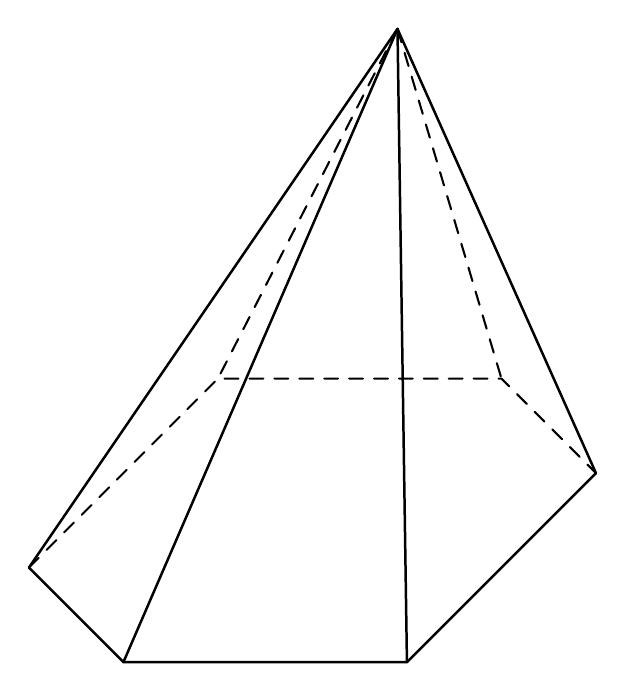
\begin{tikzpicture}[
    scale=1.2,
    line cap=round,
    line join=round,
    visible/.style={line width=0.9pt},
    hidden/.style={line width=0.75pt,dashed,dash pattern=on 5pt off 4pt}
]

% -------------------------------------------------
% Вершина пирамиды
% -------------------------------------------------
\coordinate (S) at (1.4,6.2);

% -------------------------------------------------
% Вершины правильноподобного шестиугольника в основании
% Расположены вручную по образцу рисунка
% -------------------------------------------------
\coordinate (A) at (-2.5,0.5);   % левая внешняя
\coordinate (B) at (-1.5,-0.5);  % левая передняя
\coordinate (C) at (1.5,-0.5);  % передняя центральная
\coordinate (D) at (3.5,1.5);  % правая передняя/внешняя
\coordinate (E) at (2.5,2.5);  % правая задняя
\coordinate (F) at (-0.5,2.5); % левая задняя

% -------------------------------------------------
% Основание
% -------------------------------------------------

% Видимые рёбра основания
\draw[visible] (A)--(B)--(C)--(D);

% Невидимые рёбра основания
\draw[hidden] (A)--(F)--(E)--(D);

% -------------------------------------------------
% Боковые рёбра
% -------------------------------------------------

% Видимые
\draw[visible] (S)--(A);
\draw[visible] (S)--(B);
\draw[visible] (S)--(C);
\draw[visible] (S)--(D);

% Невидимые
\draw[hidden] (S)--(F);
\draw[hidden] (S)--(E);

\end{tikzpicture}
}
